\documentclass[11pt,a4paper]{article}
\usepackage[utf8]{inputenc}
\usepackage{amsmath}
\usepackage{amsfonts}
\usepackage{amssymb}

\usepackage{graphicx}
\usepackage[colorlinks=true,citecolor=magenta,linkcolor=blue]{hyperref}

\begin{document}

\begin{center}
\begin{Large}
\textbf{NIPoPoWs under Velvet Fork\\}
\end{Large}

\end{center}

\section{Introduction}
Since the release of Bitcoin about a decade ago, the interest in cryptocurrencies has increased tremendously, while a number of other ``altcoins'' have been constructed in the meantime. Given that cryptocurrencies are starting to be considered a generally accepted means of payment and are used for everyday transactions, the issue of efficiently handling cryptocurrencies by light clients, such as smartphones, has become of great importance.

In this work, we consider the problem of optimizing light clients, or ``SPV clients'' as described in the original Bitcoin paper\cite{Nakamoto}. As blockchains are ever growing, the main setback for efficient light client applications is the processing of data amount linear to the size of the blockchain, e.g. for synchronization purposes. 

Our work is based on the construction of Non-Interactive Proofs of Proof of Work\cite{NIPoPoWs} that achieves SPV proofs of polylogarithmic portion of the blockchain size. The NIPoPoWs construction suggests a protocol update, that could be possibly implemented by a soft or a hard fork. Given the reluctancy of the community to proceed to such forks, we consider the case of a velvet fork\cite{NIPoPoWs}\cite{Zamyatin}.

Under this scope, our contributions come as follows:
\begin{itemize}
	\item We revise the security proof for NIPoPoWs suffix proof protocol and compute a concrete value for the security parameter $m$
	\item We describe an attack, that we name \textit{Chainsewing Attack}, against NIPoPoWs suffix proof construction, which is used for the light client's synchronization
	\item We suggest a patch to the NIPoPoWs protocol that eliminates the \textit{Chainsewing Attack} and prove its security
\end{itemize}

\section{Suffix Proofs}
NIPoPoWs suffix proofs are used to prove predicates that pertain to the suffix of the blockchain. For example, this is the case of light client synchronization to the longest valid chain.
 [...]
 
%\section{Model Definition and Notation}

\section{Security of NIPoPoWs Suffix Proofs} \label{proof_under_hard_fork}

In this section we provide the full security proof for the NIPoPoWs suffix proof protocol\cite{NIPoPoWs}. Apart from the proof itself (Theorem 2), we describe the definitions and lemmas being used. We try to give intuition for arguments and conclusions in each step.

Assume $t$ adversarial out of $n$ total parties, each with $q$ PoW random oracle queries per round. We define $p = \frac{T}{2^\kappa}$ the probability of a successful Random Oracle query. We will call a query to the RO $\mu$\textit{-successful} if the RO returns a value $h$ such that $h \leq 2^{-\mu}T$.

We define the boolean random variables $X_r^{\mu}$, $Y_r^{\mu}$, $Z_r^{\mu}$. Fix some round $r$, query index $j$ and adversarial party index $k$ (out of $t$). If at round $r$ an honest party obtains a PoW with $id < 2^{-\mu}T$, set $X_r^{\mu} = 1$, otherwise $X_r^{\mu} = 0$. If at round $r$ exactly one honest party obtains $id < 2^{-\mu}T$, set $Y_r^{\mu} = 1$, otherwise $Y_r^{\mu} = 0$. If at round $r$ the $j$-th query of the $k$-th corrupted party is $\mu$-successful, set $Z_{rjk}^{\mu} = 1$, otherwise $Z_{rjk}^{\mu} = 0$. Let $Z_r^{\mu} = \sum_{k=1}^t\sum_{j=1}^qZ_{rjk}^{\mu}$. For a set of rounds $S$, let $X^\mu(S) = \sum_{r \in S}X^{\mu}_r$ and similarly define $Y_S^{\mu}$, $Z_S^{\mu}$.\\

\textbf{Definition 1 (Typical Execution).} \textit{An execution of the protocol is $(\epsilon, \eta)$-typical if:}

\textbf{Block counts don't deviate.} \textit{For all $\mu \geq 0$ and any set $S$ of consecutive rounds with $\vert S \vert \geq 2^\mu \eta k$, we have:}
\begin{itemize}
\item[-] $(1-\epsilon)E[X^\mu(S)] < X^\mu(S) < (1+\epsilon)E[X^\mu(S)] $ and $(1-\epsilon)E[Y^\mu(S)] < Y^\mu(S)$
\item[-] $Z^\mu(S) < (1+\epsilon)E[Z^\mu(S)]$
\end{itemize}

\textbf{Round count doesn't deviate.} \textit{Let $S$ be a set of consecutive rounds such that $Z^\mu(S) \geq k$ for some security parameter $k$. Then $\vert S \vert \geq (1-\epsilon)2^\mu \frac{k}{pqt}$ with overwhelming probability.}

\textbf{Chain regularity.} \textit{No insertions, no copies and no predictions \cite{Backbone} have occurred.}\\

\textbf{Theorem 1 (Typicality).} \textit{Executions are $(\epsilon, \eta)$-typical  with overwhelming probability in $\kappa$.}\\

\textit{Proof.} \textbf{Block counts and regularity.} We refer to \cite{Backbone} for the full proof.

\textbf{Round count.} First, observe that for a specific round $r$ we have $Z_{rjk} \sim Bern(p)$, so for the $\mu$-level superblocks $Z_{rjk}^\mu \sim Bern(2^{-\mu}p)$ and these are jointly independent. Therefore, since for $\vert S \vert$ rounds we have $tq\vert S \vert$ adversarial RO queries, we have that $Z_S^\mu \sim \text{Bin}(tq \vert S \vert, 2^{-\mu}p)$. So $tq \vert S \vert \sim \text{NB}(Z_S^\mu, 2^{-\mu}p)$. Negative Binomial distribution is defined as $\text{NB}(r, p')$ and, for our purposes, expresses the number of trials in a sequence of independent and identically distributed Bernoulli trials before a specified $(r)$ number of successes occurs. The expected total number of trials of a negative binomial distribution with parameters $(r, p')$ is $r/p'$. To see this, imagine an experiment simulating the negative binomial performed many times, that is a set of trials is performed until $r$ successes occur. Consider you perform $n$ experiments of total $N$ trials. Now we would expect $Np' = nr$, so $N/n = r/p'$. See that $N/n$ is just the average number of trials per experiment. So we have $E[tq \vert S \vert] = \frac{Z^\mu_S}{2^{-\mu}p} \Rightarrow E[\vert S \vert] = 2^\mu \frac{Z^\mu_S}{tqp}$. So if $Z^\mu(S) \geq k$ then $E[\vert S \vert] \geq 2^\mu \frac{k}{tqp}$. Applying a tail bound to the negative binomial distribution, we obtain that $\text{Pr}[\vert S \vert < (1 - \epsilon)E(\vert S \vert)] \in \Omega(\epsilon^{2}m)$.  \\

\textbf{Lemma 1.} \textit{Suppose S is a set of consecutive rounds $r_1 ... r_2$ and $C_B$ is a chain adopted by an honest party at round $r_2$ of a typical execution. Let $C^{B}_{S} = \{$ b $\in C_B:$ b was generated during $S\}$. Let $\mu_A, \mu_B \in \mathbb{N}$. Suppose $C^{B}_{S}\uparrow^{\mu_B}$ is good. Suppose $C'_A$ is a $\mu_A$-superchain containing only adversarially generated blocks generated during S and suppose that $\vert C'_A \vert \geq k$. Then $2^{\mu_A} \vert C'_A \vert <  2^{\mu_B} \vert    C^{B}_{S}\uparrow^{\mu_B}\vert $. }\\

\textit{Proof.} From $\vert C'_A \vert \geq k$ we have that $\vert Z^{\mu_A}_S \vert \geq k$. Applying Theorem 1, we conclude that $\vert S \vert \geq (1-\epsilon')2^{\mu_A} \frac{\vert C'_A \vert}{pqt}$. Applying the Chain Growth theorem \cite{Backbone} we obtain $\vert C_{B}^S \vert \geq (1 - \epsilon)f \vert S \vert$. But from the goodness of $C_{B}^S \uparrow^{\mu_B}$, we know that $\vert C_{B}^S\uparrow^{\mu_B} \vert \geq (1 - \delta)2^{-\mu_B} \vert C_{B}^S \vert $. So we have $\vert C_{B}^S\uparrow^{\mu_B} \vert \geq (1 - \delta)2^{-\mu_B} (1 - \epsilon)f \vert S \vert $ and follows that $\vert C_{B}^S\uparrow^{\mu_B} \vert \geq (1 - \delta)2^{-\mu_B} (1 - \epsilon)f (1-\epsilon')2^{\mu_A} \frac{\vert C'_A \vert}{pqt} $. Consequently we have that $2^{\mu_A} \vert C'_A \vert \leq \frac{pqt}{(1- \delta)(1-\epsilon)(1-\epsilon')f} 2^{\mu_B} \vert C_{B}^S\uparrow^{\mu_B} \vert $.   \\

So, according to the above equation we have that $2^{\mu_A} \vert C'_A \vert <  2^{\mu_B} \vert    C^{B}_{S}\uparrow^{\mu_B}\vert $ considering that honest  majority assumption holds, specifically considering that $ \frac{pqt}{f} \approx \frac{t}{n-t} \leq 1 $ .\\

\textbf{Definition 2 (Adequate level of honest proof).} \textit{Let $\pi$ be an honestly generated proof constructed upon some adopted chain $C$ and let $b \in \pi $. Then $\mu'$ is defined as $\mu' = \max \{ \mu: \vert \pi\{b:\}\uparrow^{\mu} \vert \geq \max( m+1, (1-\delta)2^{-\mu} \vert \pi\{b:\}\uparrow^{\mu}\downarrow \vert )   \}$}.
\textit{We call $\mu'$ the adequate level of proof $\pi$ with respect to block b with security parameters $\delta$ and m. Note that the adequate level of a proof is a function of both the proof $\pi$ and the chosen block b.}\\

\textit{Intuitively, adequate is the level $\mu'$ of a proof $\pi$ for a block b if there are at least $m$ blocks after b in $\pi$ under the condition that there is good chain quality for this level, meaning that there are at least so many blocks at this level as expected considering the number of 0-level blocks.\\ 
NOTE: adequate level is mostly useful for Claim 1a of the Security Proof (Theorem 2).}\\

\textbf{Lemma 2.} \textit{Let $\pi$ be some honest proof generated with security parameters $\delta$, m. Let C be the underlying chain, $b \in C$ be any block and $\mu'$ be the adequate level of the proof with respect to b and the same security parameters.\\Then $C\{b:\}\uparrow^{\mu'} = \pi\{b:\}\uparrow^{\mu'}$.}\\

\textit{Proof.} $ \pi\{b:\}\uparrow^{\mu'} \subseteq C\{b:\}\uparrow^{\mu'}$ is trivial. For the converse, we have that in the iteration of the \emph{Prove for loop}\cite{NIPoPoWs} with $\mu = \mu^*$, the block stored in variable $B$ preceds $b$ in $C$.

Note that the Prover's for loop iterates over all levels in the interlink structure, and places in the proof all of the blocks that are of the corresponding level and succeed $B$ in $C$. 

Suppose $\mu = \mu^*$ is the first \emph{for} iteration during which the property is violated. This cannot be the first iteration since $B = C[0]$ and Genesis precedes all blocks. By induction hypothesis we see that during the iteration $\mu = mu^* + 1$, $B$ preceded $b$. From the definition of $\mu'$ we know that $\mu'$ is the highest level for which $\vert \pi\{b:\}\uparrow^{\mu} \vert \geq \max( m, (1-\delta)2^{-\mu} \vert \pi\{b:\}\uparrow^{\mu}\downarrow \vert ) $. 

Hence, this property cannot hold for $\mu^* > \mu$ and therefore $\vert \pi\{b:\}\uparrow^{\mu} \vert < m$ or $\neg$local-good$_\delta(\pi\{b: \}\uparrow \mu^*[1:], C, \mu^*)$.

In case local-good is violated, variable $B$ remains unmodified and the induction step holds. If local-good is not violated, then $ \vert \pi\{b:\} \uparrow^{\mu^*}[1:] \vert < m$ and so $\pi\uparrow^{\mu^*}[-m]$, which is the updated value of $B$ at the end of $\mu^*$ iteration, precedes $b$.\\

\textbf{Lemma 3.} \textit{Suppose the verifier evaluates $\pi_A \geq \pi_B$ in a protocol interaction where B is honest and assume during the comparison that the compared level of the honest party is $\mu_B$. Let $b = LCA(\pi_A, \pi_B)$ and let ${\mu}'_B$ be the adequate level of $\pi_B$ with respect to b. Then ${\mu}'_B \geq \mu_B$.}\\

\textit{Proof.} Because $\mu_B$ is the compared level of the honest party, from the definition of the $\geq_m$ operator, we have $2^{\mu_B} \vert \pi\{b:\}\uparrow^{\mu_B} \vert > 2^{{\mu}'_B} \vert \pi\{b:\}\uparrow^{{\mu}'_B} \vert $. This is true, otherwise the Verifier would have chosen level $\mu'_B$ as level of comparison. The proof is by contradiction. Suppose $\mu'_B < \mu_B$. 
By definition, $\mu'_B$ is the maximum level such that $\vert \pi_B\{b:\}\uparrow^\mu [1:] \vert \geq max(m, (1-\delta)2^{-\mu}\vert \pi_B\{b:\}\uparrow^\mu [1:]\downarrow \vert)$, 
therefore $\mu_B$ does not satisfy this condition. 
But we know that $\vert \pi_B\{b:\}\uparrow^\mu [1:] \vert > m$ because $\mu_B$ was selected by the Verifier. 
Therefore $ 2^{\mu_B} \vert \pi\{b:\}\uparrow^{\mu_B} \vert < (1-\delta)\vert C\{b:\}\vert $. \\
But also $\mu'_B$ satisfies goodness, so $ 2^{\mu'_B} \vert \pi\{b:\}\uparrow^{\mu'_B} \vert > (1-\delta)\vert C\{b:\}\vert $.\\ From the last two equations we obtain $ 2^{\mu_B} \vert \pi\{b:\}\uparrow^{\mu_B} \vert < 2^{\mu'_B} \vert \pi\{b:\}\uparrow^{\mu'_B} \vert$ which contradicts the initial equation.\\

@To Be Discussed: would the verifier ever choose a non-adequate level for proof comparison? \\
Intuitively the above Lemma says: the comparison level chosen by the Verifier can be no other than the adequate level in respect to block b ($LCA(\pi_A, \pi_B)$), since any other choice would be a level of non-good quality, because of the definition of the adequate level. A level of non-good quality would contain less PoW than that of the adequate level for the range of interest $C\{b:\}$. \\


\textbf{Theorem 2. (Security)}\textit{Assuming honest majority, the non-interactive proofs-of-proof-of-work construction for computable $\kappa$-stable monotonic suffix-sensitive predicates is secure with overwhelming probability in $\kappa$.}\\

By contradiction. Let $Q$ be a $\kappa-$stable monotonic suffix-sensitive chain predicate. Assume NIPoPoWs on $Q$ is insecure. Then, during an execution at some round  $r_3$, $Q(C)$ is defined and the verifier $V$ disagrees with some honest participant. Assume the execution is typical. $V$ communicates with adversary $A$ and honest prover $B$. The verifier receives proofs $\pi_A, \pi_B$. Because $B$ is honest, $\pi_B$ is a proof constructed based on underlying blockchain $C_B$ (with $\pi_B \subseteq C_B$), which $B$ has adopted during round $r_3$ at which $\pi_B$ was generated. Furthermore, $\pi_A$ was generated at round $r'_3 \leq r_3$.

The verifier outputs $\neg Q(C_B)$. Thus it is necessary that $\pi_A \geq \pi_B$. We show that $\pi_A \geq \pi_B$ is a negligible event. 

Let $b = LCA(\pi_A, \pi_B)$. Let $b^\star$ be the most recently honestly generated block in $C_B$ preceding $b$. Note that $b^\star$ necessarily exists because Genesis is honestly generated. Let the levels of comparison decided by the verifier be $\mu_A$ and $\mu_B$ respectively. Let $\mu'_B$ be the adequate level of proof $\pi_B$  with respect to block $b$. Call $\alpha_A = \pi_A \uparrow^{\mu_A}\{b:\}$, 
$\alpha'_B = \pi_B \uparrow^{\mu'_B}\{b:\}$.

%%ANDRI:
Note that we consider the parts of the proofs succeeding block $b$ the decisive ones for the verifier's choice. This is to adversary's advantage, since the parts preceding this block demonstrate the proof-of-work contained in the common (sub)chain, thus the adversary could only include equal or less proof-of-work in her proof for this part of the chain.

We will now show three successive claims: First, $\alpha_A$ and $\alpha'_B \downarrow$ are mostly disjoint. Second, $a_A$ contains mostly adversarially generated blocks. And third, the adversary is able to produce this $a_A$ with negligible probability.

Let $\alpha_A = k_1 + k_2 + k_3$ and let $k_1, k_2, k_3$ be as defined in the following Claims.

\textbf{Claim 1:} $\alpha_A, \alpha'_B\downarrow$ are mostly disjoint. We show this by taking the two possible cases for the relation of $\mu_A$, $\mu'_B$.\\
\textit{\underline{Claim 1a}:} If $\mu'_B \leq \mu_A$ then they are completely disjoint. In such a case of inequality, every block in $\alpha_A$ would also be of lower level $\mu'_B$. Applying Lemma 2 to $C\{b:\}\uparrow^{\mu'_B}$  we see that $C\{b:\}\uparrow^{\mu'_B} = \pi\{b:\}\uparrow^{\mu'_B}$. Subsequently, any block in $\pi_A\uparrow^{\mu_A}\{b:\}[1:]$ would also be included in proof $\alpha'_B$, but $b=LCA(\pi_A, \pi_B)$ so there can be no succeeding block common in $\alpha_A, \alpha'_B$. \\
\\
\textit{\underline{Claim 1b}:} If  $\mu'_B > \mu_A$ then $\vert \alpha_A[1:] \cap \alpha'_B\downarrow[1:] \vert = k_1 \leq 2^{\mu'_B - \mu_A}$.\\
%% possibly unnecessary sentence%%%%%
First observe that because the adversary is winning $2^{\mu_A} \vert \alpha_A \vert > 2^{\mu'_B} \vert \alpha'_B \vert \geq 2^{\mu'_B} m \Rightarrow \vert \alpha_A \vert > 2^{\mu'_B - \mu_A}m$.
%%%%%%%%%%%%%%%%%%%%%%%%%%%%%%%%%%%%%%%%%%
Let's call $b_1$ the first block in $\alpha'_B$ after block b.
Suppose for contradiction that $k_1 > 2^{\mu'_B - \mu_A}$.  Since $C_B^{\mu'_B}$ is of good chain quality, this would mean that block $b_1$, of level $\mu'_B$, also exists in $\alpha_A$ since it is of level $\mu_A$ too. But $b_1$ cannot exist in both $\alpha_A, \alpha'_B$ since $\alpha_A \cap \alpha'_B = \emptyset$ by definition.  \\


From Claim $1a$ and Claim $1b$, we conclude that there are $\vert \alpha_A \vert - k_1$ blocks after block $b$ in $\alpha_A$ which do not exist in $\alpha_B\downarrow$. We now set $b_2 = LCA(C_B, \alpha_A)$. This makes $b_2$ the last block before the fork point at the 0-level chain included in the adversary's proof.\\

Intuition: in this case the common blocks of $\alpha_A, \alpha'_B\downarrow$ may only be blocks of level $\mu_A$ which precede the first $\mu'_B$ block appearing in $\alpha'_B$. If this block of level $\mu'_B$ was common, it could also be included in $\alpha_A$. If it is included this would be the LCA of $\alpha_A, \alpha'_B$. If it is not, then the adversary could no more include blocks from the common part of chain $C_B$ in her proof since they no longer form a valid chain in $\alpha_A$. The quantity $2^{\mu'_B - \mu_A}$ means: in the range between two consequent $\mu'_B$-level blocks, we have $n = 2^{\mu'_B}$ 0-level blocks and, thus, $2^{-\mu_A}n = 2^{\mu'_B - \mu_A}$ blocks of $\mu_A$-level. \\

\textbf{Claim 2:} At least $k_3$ superblocks of $\alpha_A$ are adversarially generated. We show this by showing that $\alpha_A[k_1 + k_2 + 1:]$ contains no honestly generated blocks. Suppose for contradiction that the block $\alpha_A[i]$ for some $i \geq k_1 + k_2 + 1$ was honestly generated. This means that an honest party adopted the chain $\alpha_A[:i - 1]\downarrow$ at some round $r_2 \leq r_3$. Because of the way honest parties adopt chains, the superchain $\alpha_A[:i - 1]$ has an underlying properly constructed 0-level anchored chain $C_A$ such that $\alpha_A[:i - 1] \subseteq C_A$. Let $j$ be the index of block $b_2$ within $\alpha_A$, $j_\downarrow$ be the index of block $b_2$ within $C_A$ and $k_{2\downarrow} = \vert \alpha_A[j:j+k_2]\downarrow\vert$. See Figure \ref{fig:proof} for a demonstration. Observe that $\vert C_A[:\{\alpha_A[i-1]\}] \vert \geq \vert C_A[:{j_\downarrow}+k_{2\downarrow}] \vert$, while $C_A[j_\downarrow:j_\downarrow + k_{2\downarrow}] \npreceq C_B$ as proved in Claim 1. But $C_A$ was adopted by an honest party at round $r_2$, which is prior to round $r_3$ during which $C_B$ was adopted by an honest party B. This contradicts the Common Prefix\cite{Backbone} with parameter $k_{2\downarrow}$. It follows that with overwhelming probability in $k_{2\downarrow}$, the $k_3 = \vert \alpha_A \vert - k_2 - k_1$ last blocks of the adversarial proof have been adversarially generated.\\

\begin{figure}[h]
	\begin{center}
		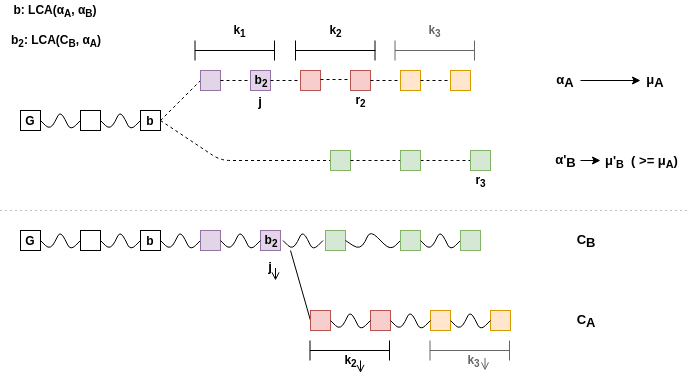
\includegraphics[scale=0.5]{figures/proof.png}
	\end{center}
	\caption{\textit{Two competing proofs at different levels. At the bottom the corresponding 0-level chains are represented.}}
	\label{fig:proof}
\end{figure}

Intuitively: Because of Common Prefix on $k_{2\downarrow}$ parameter, where $k_{2\downarrow} = \vert \alpha_A[j:j+k_2]\downarrow\vert$, where $E[k_{2\downarrow}] = 2^{\mu_A}k_2$, there can be no honest party adopting $C_A$ at any round $i \geq k_1 + k_2 + 1$. \\

From these two Claims we have that $k_1$ blocks in $\alpha_A$ are blocks of the common zero-level chain, while $k_2$ blocks are blocks after the fork point at the zero-level chain. Subsequently, $k_2$ is subject to the Common Prefix $\kappa-$parameter limitations as described in the Backbone paper\cite{Backbone}.\\

\textbf{Claim 3:} Adversary $A$ is able to produce $\alpha_A$ that wins against $\alpha_B$ with negligible probability.

Let $b'$ be the latest honestly generated block in $a_A$, or $b' = b^*$ if no such block exists in $a_A$. Let $r_1$ be the round when $b'$ was generated. Consider the set $S$ of consecutive rounds $r_1..r_3$. Every block in $\alpha_A[-k_3:]$ has been adversarially generated during $S$ and $\vert \alpha_A[-k_3:] \vert = \vert \alpha_A\{b':\} \vert = k_3$. $C_B$ is a chain adopted by an honest party at round $r_3$ and filtering the blocks by the rounds during which they were generated to obtain $C_B^S$, we see that if $b''$ is the most recently generated block in $\alpha_B$ in a round $r \leq r_1$, then $C_B^S = C_B\{ b'': \}$. But $C_B^S \uparrow^{\mu'_B}$ is good with respect to $C_B^S$. Applying Lemma 1, we obtain that with overwhelming probability  $2^{\mu_A} \vert \alpha_A\{b':\} \vert < 2^{\mu'_B} \vert C_B^S \uparrow^{\mu'_B} \vert$, which is equal to

\begin{equation}
2^{\mu_A} \vert \alpha_A\{b':\} \vert < 2^{\mu'_B} \vert \alpha'_B\{b'':\} \vert
\end{equation} 

since $\alpha'_B$ contains all the $\mu'_B$-level blocks in $C_B^S$. \\


In order to complete the proof, let us know consider $\alpha_A^{k_1}$, $\alpha_A^{k_2}$, $\alpha_A^{k_3}$ the parts of $\alpha_A$ where the $k_1$, $k_2$, $k_3$ blocks reside and 
$\alpha_B^{k_1}$, $\alpha_B^{k_2}$, $\alpha_B^{k_3}$ the parts of $\alpha_B$ containing blocks generated in the corresponding round sets as illustrated in Figure \ref{fig:claim3}.

\begin{figure}[h]
	\begin{center}
		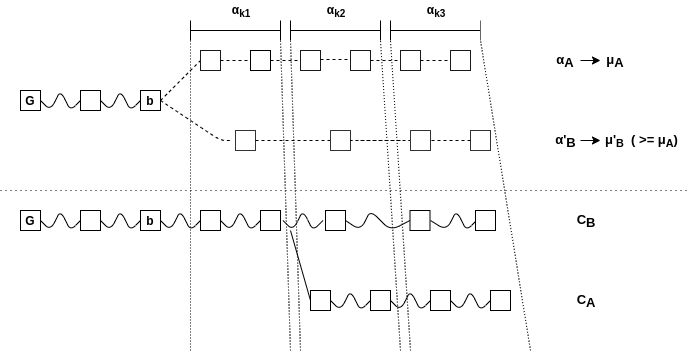
\includegraphics[scale=0.5]{figures/claim3.png}
	\end{center}
	\caption{\textit{The three round sets in two competing proofs at different levels. The vertical dashed lines denote the area of interest, across proofs and chains, corresponding to each round set. At the bottom the corresponding 0-level chains are represented.}}
	\label{fig:claim3}
\end{figure}

Subsequently to the above Claims we have that:

Because of the common underlying chain in the first round set:
\begin{equation} \label{eq_round_set_1}
2^{\mu_A} \vert \alpha_A^{k_1} \vert \leq 2^{\mu'_B} \vert \alpha'{_B^{k_1}} \vert
\end{equation}

Because of the adoption by an honest party of chain $C_B$ at a later round $r_3$, we have for the second round set:
\begin{equation} \label{eq_round_set_2}
2^{\mu_A} \vert \alpha_A^{k_2} \vert \leq 2^{\mu'_B} \vert \alpha'{_B^{k_2}} \vert
\end{equation}

Because of Equation (1), we have for the third round set:
\begin{equation} \label{eq_round_set_3}
2^{\mu_A} \vert \alpha_A^{k_3} \vert < 2^{\mu'_B} \vert \alpha'{_B^{k_3}} \vert
\end{equation}

So we have

\begin{equation*}
2^{\mu_A} ( \vert \alpha_A^{k_1} \vert + \vert \alpha_A^{k_2} \vert + \vert \alpha_A^{k_3} \vert ) < 2^{\mu'_B} ( \vert \alpha'{_B^{k_1}} \vert + \vert \alpha'{_B^{k_2}} \vert + \vert \alpha'{_B^{k_3}} \vert)
\end{equation*}

and finally 
\begin{equation}
2^{\mu_A} \vert \alpha_A \vert < 2^{\mu'_B} \vert \alpha'{_B} \vert
\end{equation}


Therefore we have proven that $2^{\mu'_B} \vert \pi_B \uparrow^{\mu'_B} \vert > 2^{\mu_A} \vert \pi_A^{\mu_A} \vert$. From the definition of $\mu_B$, we know that $2^{\mu_B} \vert \pi_B \uparrow^{\mu_B} \vert > 2^{\mu'_B} \vert \pi_B \uparrow^{\mu'_B} \vert$ because it was chosen $\mu_B$ as level of comparison by the Verifier. So we conclude that $2^{\mu_B} \vert \pi_B \uparrow^{\mu_B} \vert > 2^{\mu_A} \vert \pi_A \uparrow^{\mu_A} \vert$.

\begin{flushright}
$\square$
\end{flushright}

It remains to compute the security parameter $m$ that guarantee that all the above hold true in every implementation. It suffices to compute a security parameter value for each set of rounds $k_1, k_2, k_3$, so that the proof equations \ref{eq_round_set_1}, \ref{eq_round_set_2}, \ref{eq_round_set_3} hold and then sum these values to obtain parameter $m$.

In the first set of rounds, for the first $k_1$ blocks in $\alpha_A$, we only need 1 block included in $\alpha_B$ for the part of the proof described in Equation \ref{eq_round_set_1}. In the second set of rounds we need $2^{-\mu_B}\kappa$ blocks for the part of the proof described in Equation \ref{eq_round_set_2}, just as it directly results from the Common Prefix property. In order to make $m$ independent of any specific level it suffices to consider the upper bound of $\kappa$ blocks for this set of rounds. In the last set of rounds we need at least $\kappa$ adversarially generated blocks in $\alpha_A^{k_3}$ so that Lemma 1 is applicable. Since we assume honest majority, obliging to at least $\kappa$ blocks for this set of rounds suffices to guarantee for Equation \ref{eq_round_set_3}.

So, we finally conclude to the following upper bound for the value of the
 security parameter:
\begin{equation}
m = 2\kappa + 1 
\end{equation}
 
\section{NIPoPoWs under Velvet Fork}

\subsection{The Chainsewing Attack}
We  will now describe an explicit attack against the NIPoPoW suffix proof construction under a velvet fork. Note that since the protocol is implemented under a velvet fork, any adversarial block that is mined in the proper way except containing false interlink data structure will be accepted as valid. A false interlink may contain invalid pointers, for example pointers to superblocks of a fork chain, as shown in Figure \ref{fig:false_interlink}.
Taking advantage of this fact, an adversary maintaining a fork chain could produce suffix proofs that claim blocks of the chain adopted by an honest player as her own. The attack is described in detail in the following.

\begin{figure}[h]
	\begin{center}
		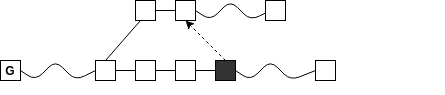
\includegraphics[scale=0.6]{figures/false_interlink.png}
	\end{center}
	\caption{\textit{Example of false interlink structure of an adversarial block, coloured black, in an honest player's chain. The dashed arrow is a pointer to a fork chain superblock included in the interlink.}}
	\label{fig:false_interlink}
\end{figure}

Assume that chain $C_B$ was adopted by an honest player B and chain $C_A$, a fork of $C_B$ at some block, maintained by an adversary A. Assume the adversary wants to produce a suffix proof in order to attack an honest light client to have him adopt chain $C_A$. In order to achieve this, the adversary needs to include a greater amount of PoW in her suffix proof, $\pi_A$, in comparison to the honest player's proof, $\pi_B$, so as to achieve $\pi_A \geq_m \pi_B$. For this she produces some blocks in chains $C_A$ and $C_B$ containing false interlink pointers which will allow for claiming blocks of chain $C_B$ as of chain $C_A$ in her suffix proof.

The general setting of this attack is represented in Figure \ref{fig:generic_attack}. The dashed arrows represent interlink pointers of some level $\mu_A$. Starting from the most recently mined block in the adversary's fork chain and following the interlink pointers a chain is formed which consists the adversary's suffix proof. Blocks of both chains are included in this proof and a verifier could not distinguish the false interlink pointers forming this chain proof and, as a result, would consider it a valid proof. 

\begin{figure}[h]
	\begin{center}
		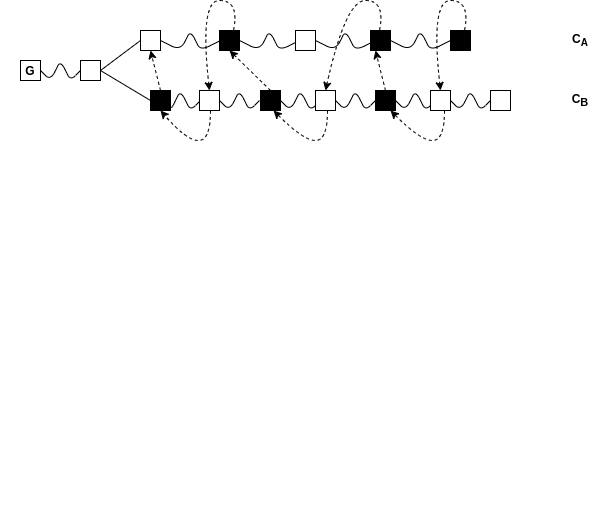
\includegraphics[scale=0.55]{figures/generic_chainsewing_attack.png}
	\end{center}
	\caption{\textit{Generic Chainsewing Attack. $C_B$ is the chain of an honest player and $C_A$ the adversary's chain. Blocks generated by the adversary are colored black. Dashed arrows represent interlink pointers included in the adversary's suffix proof. Wavy lines imply one or more blocks.}}
	\label{fig:generic_attack}
\end{figure}

As the generic attack scheme may seem a bit complicated we will now describe a more specific attack case. Consider that the adversary acts as described below. 
Assume that the adversary chooses to attack at some level $\mu_A$. As shown in Figure \ref{fig:attack} she first generates a superblock $b'$ in her fork chain $C_A$ and a superblock $a'$ in the honest chain $C_B$ which are connected via an invalid interlink pointer from $a'$ to $b'$. As argued earlier, block $a'$ will be accepted as valid in the honest chain $C_B$ despite the false pointers in the interlink data structure. After that the adversary may mine on chain $C_A$ or $C_B$, or not mine at all. At some point she produces a block $a$ in $C_A$ containing an interlink pointer to a block $b$ of the honest player's chain $C_B$. Because of the way blocks are generated by updated honest miners there will be successive interlink pointers leading from block $b$ to block $a'$. Thus following the interlink pointers a chain is formulated which connects $C_A$ blocks $a$ and $b'$ and contains an arbitrarily large part of the honest player's chain $C_B$.

At this point the adversary will produce a suffix proof for chain $C_A$ containing the subchain $C\{ab\} \cup C\{b:a'\} \cup C\{a':b'\}$. Notice that following the interlink pointers constructed in such a way, a light client perceives $C\{ab\} \cup C\{b:a'\} \cup C\{a':b'\}$  as a valid chain.

\begin{figure}[h!]
	\begin{center}
		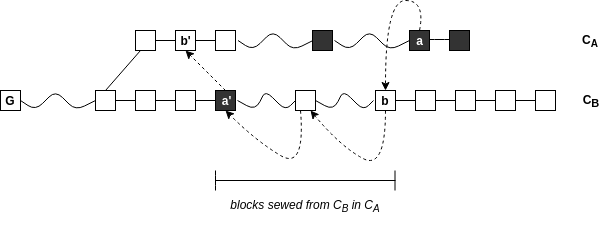
\includegraphics[scale=0.55]{figures/chainsewing_attack.png}
	\end{center}
	\caption{\textit{Chainsewing Attack. The chain at the bottom represents the chain of an honest player, $C_B$, while the above one is the adversarial fork, $C_A$. Blocks generated by the adversary are colored black. Dashed arrows represent interlink pointers included in the suffix proof by the adversary. Wavy lines imply one or more blocks. Firm lines imply the previousId relationship between two sequential blocks.}}
	\label{fig:attack}
\end{figure}

In this attack the adversary uses false interlink pointers to ``sew`` portions of the chain adopted by an honest player to her own fork. This remark justifies the name given.  

Note that in order to make this attack successful, the adversary has to produce only a few superblocks which let her arrogate an arbitrary large number of blocks of an honest player's chain, while she can mine for her own fork chain. Thus intuitively we expect this attack to succeed with overwhelming probability.

@TODO

Needs to be proven. It is not obvious that the attacker will succeed in high probability, since the most important adversarially generated blocks , $a$ and $a'$, set a limit to the adversarial blocks produced in parallel to the honest blocks of subchain $C\{ab\} \cup C\{b:a'\} \cup C\{a':b'\}$ and can take part in the suffix proof.

\subsection{Protocol Update}

In order to eliminate the Chainsewing Attack we propose an update to the NIPoPoWs protocol under velvet fork. The core problem is that in her suffix proof the adversary is able to claim not only blocks of the fork chain,  which are in majority adversarially generated due to the Common Prefix property, but also an arbitrarily long part of the chain adopted by an honest player. Since blocks containing false interlink pointers are accepted as valid, the verifier cannot distinguish blocks that actually belong in a chain from blocks that only seem to belong in the same chain because they are pointed to via a false interlink pointer. \\

%% first reference to 1/3 adversary
These facts make it possible to provide a secure solution for the velvet fork conditions only under the assumption of adversary of $1/3$ of the total hashing power. This claim is described and discussed in the following subsection.

\subsubsection{Impossibility of a protocol for (1/2)-bounded adversary}
During our study on the problem we failed to prove the security of several protocol constructions under $(\frac{1}{2})$-bounded adversary. We finally concluded that such a secure NIPoPoWs construction is impossible under velvet fork conditions. Though it is hard to provide a typical proof for this claim, as one should consider any possible construction, in this section we will try to argue for it. 

\textbf{Claim:} \textit{Assume $t$ adversarial out of total $n$ parties. There is no construction for NIPoPoWs suffix proofs under velvet fork conditions, which is secure for every adversary $t$, such that $\dfrac{t}{n-t} < \delta$.}

\textit{Discussion.} As explained earlier, since the adversary may use the interlink structure so as to include pointers to arbitrary blocks,  she may construct her own chain history utilizing the false pointers included in the blocks she herself generates. Such an example is given in Figure \ref{fig:generic_attack}.

Let us consider a construction $p$ which allows for NIPoPoWs suffix proofs under velvet fork and is secure for the underlined conditions. In order $p$ to have a chance for being secure, it should be possible to challenge the submitted proofs, so that an honest player can contest against an inconsistent proof. Note that the same power to challenge any submitted proof is also provided to the adversary.



Now assume an adversary of $ \frac{n}{3} < t < \frac{n}{2} $. Then, as explained in the Backbone and Selfish Mining papers \cite{Backbone}\cite{selfish_mining} it is possible for the adversary to maintain the longest valid chain of less than $50\%$ chain quality in favor of adversarially generated blocks. This is illustrated in Figure \ref{fig:selfish_mining_pie}. 

\begin{figure}[h!]
	\begin{center}
		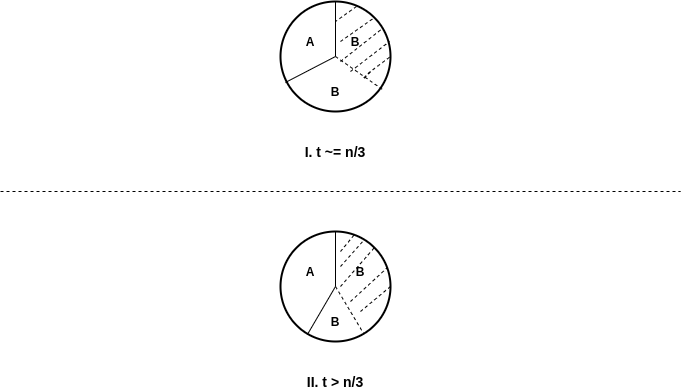
\includegraphics[scale=0.55]{figures/selfish_mining_pie.png}
	\end{center}
	\caption{\textit{Total  of adversarially and honestly generated blocks distribution during a round set S. \textbf{A} stands for blocks mined by the adversary while \textbf{B} for blocks mined by honest parties. Lined out parts denote mined blocks that were defeated by adversarially mined ones in the same round due to selfish mining. The rest denote blocks placed in the chain adopted by honest parties. \textbf{I.} With $t = n/3$, $50\%$ of the total blocks are adversarially generated in the worst case scenario. \textbf{II.} With $t > n/3$, more than half of the total blocks are adversarially generated in the worst case scenario.}}
	\label{fig:selfish_mining_pie}
\end{figure}

Observe that the property that is violated in the described attack is the $prevId$ relation among sequential blocks and cannot be validated under our working hypothesis conditions. However since the main purpose of our work is to achieve succinctness, we consider that 0-level reliability provided by the \textit{prevId} relations is not viable in order to contest adversarial proofs that utilize false interlink pointers. This is obvious in part II of Figure \ref{fig:selfish_mining_pie}, since a chain of bad quality could force a contesting proof proportional to the length of the chain, if it was to utilize the 0-level $prevId$ pointers. We thus consider that we should mostly rely on the information given by the interlink data structure as far as the validity of any proof is concerned so as to keep our protocol construction efficient.

Now assume, to honest party's favor, that it is both possible and efficient to inspect the whole chain history that each block is commited to via its interlink pointers. Keep in mind that an adversary can keep a consistent chain considering the interlink pointers by using only her own mined blocks and, at the same time, these blocks may overwhelm the honestly generated ones. In protocol $p$ it should be decided  under what policy an honest party generates blocks and constructs suffix proofs. A decision should be made for block generation:
\begin{enumerate}
\item interlink data are neutral as for adversarially and honestly generated blocks or 
\item interlink data point out inconsistent blocks, meaning blocks with incorrect interlinks
\item interlink data exclude inconsistent blocks from being part of the valid chain the super-pointers form
\end{enumerate}

Now let's discuss the above choices. 
In the first case the arguments that an honest player could provide against an inconsistent proof could only be based on the 0-level pointers. Such a contesting proof should at least provide the 0-level subchain of length equal to the following: starting from a block included in the suffix proof but is not a block of the chain until the closest block included in the suffix proof and is a valid block of the chain. This means that contesting proofs are expected to be of length $2^\mu$ where $\mu = log(|C|)$, and subsequently are of complexity $\mathcal{O}(|C|)$ which ruins the succinctness of our protocol.

In the second case an honest party could utilize this extra information provided in the interlink to prove an inconsistent proof wrong. However, keep in mind that the adversary could make such claims too. So, a claim of inconsistency for a specific included block should be followed by a proof of its inconsistency. So we fall to the previous case, where the contesting proofs are unacceptable efficiency-wise.

In the third case we demand from the honest players to validate the interlink structures of the blocks in the chain and exclude the inconsistent ones from the chain history that the interlinks provide. In this way we possibly could provide contesting proofs using information only from the interlinks thus keeping our proofs succinct. This solution would result to two different chain histories considering the interlink pointers: the one of the honest parties that includes only blocks with valid interlinks, and the one of the adversary which may form her own history of invalid blocks but could not include honest blocks if at least one invalid block participates. This solution seems to bring us to a notable trade-off point. On the one hand we manage to uncouple from the 0-level blocks. On the other hand, we compromise that honest players cannot use valid adversarially generated blocks in their proof, while the adversary cannot include honestly generated blocks in her proofs if inconsistent blocks are also included. This solution could not work properly for $(\frac{1}{2})$-bounded adversary though. The reason lies in the bad chain quality as pointed out earlier and shown in Figure \ref{fig:selfish_mining_pie}. If the adversary  could create his own chain history including inconsistent blocks, then she could easily construct a suffix proof that wins over an honest one because the majority of the blocks included in the chain could be adversarial with high probability. 

We conclude that such a protocol could not exist for $(\frac{1}{2})$-bounded adversary.





\subsubsection{Solution for (1/3)-bounded adversary}
The vulnerability that makes this attack possible is the acceptance of blocks containing false interlink pointers. Since we operate under a velvet fork we cannot eliminate such blocks, but we need, however, to restrict the adversary from being able to claim portion of another chain as part of her own fork chain. 
The key observation on the Chainsewing Attack is that the adversary needs at least one adversarially generated block in an honest player's chain (block $a'$), in order to create a path of superpointers connecting blocks of two, or more, diverse chains. The final proof chain will make use of this crossing point and may contain both honest or adversarial blocks. 
%% intuitive reference to 1/3 adversary
In case the proof contains only adversarial blocks, the attack cannot harm security for an adversary of less than $1/3$ hashing power. This fact will be clear in the security proof section. In short, it is true that an adversary of $1/3$ of the total hashing power can competitive in the longest valid chain as of chain quality. This means that such an adversary could manage to maintain $50\%$ of the total blocks included in the longest valid chain by following the Selfish Mining strategy\cite{selfish_mining}. An attacker of more than $1/3$ hashing power would dominate as of total hashing power expressed in mined blocks in the chain, while the inverse would be true for an attacker of less hashing power than this threshold.
So in order to be successful, the attacker needs to ``sew`` honestly generated blocks. Thus there will be at least one honest block in the superblock path connecting blocks $a$ and $a'$, which points to an adversarial block containing false interlink or, by induction, pointing to a block containing false interlink.

The idea is to ban all blocks generated by honest players from participating in this superblock path. In this way the adversary could not misuse hashing power of the honest players and the sewed blocks could only be adversarially generated, thus the attack would never succeed for an adversary of less than $1/3$ of the total hashing power. 
We describe a protocol patch that operates as follows. The NIPoPoW protocol under velvet fork works as usual but each miner constructs a block's interlink excluding the blocks with false interlink (except the pointers of level 0). In this way, blocks containing false interlink pointers are integrated in the chain but are not taken into consideration when updating the interlink structure for the next block to be mined. No honest block could now point to an adversarial superblock that may act as the passing point to the fork chain in an adversarial suffix proof. 
After this protocol update the adversary is only able to inject adversarially generated blocks from the chain adopted by an honest party to her own fork. This is illustrated in Figure \ref{fig:injection}.
Since an updated honest miner will not include interlink pointers to adversarially generated blocks with incorrect interlinks, these adversarially generated blocks cannot participate in an honestly generated suffix proof, while they may participate in an adversarially suffix proof for the adversary's fork chain. Consequently, as far as the hashing power included in a suffix proof is concerned, these blocks can be conceived as belonging in the adversary's fork chain. 
Hence, the following two Lemmas come as results from the suggested protocol update.\\
\textbf{Lemma 1.} A suffix proof constructed by an honest player cannot contain any adversarially generated block with incorrect interlink structure.\\
\textbf{Lemma 2.} Consider $C_B, C_A$ the 0-level chains adopted by an honest player and the adversary at some round $r$. Let block $b = LCA(C_A, C_B)$. A suffix proof $\pi_A$ that contains blocks of $C_A$ constructed by an adversary is subject to the following: i) for the blocks included by the common subchain $C_B\{:b\}$ either they are honestly generated or once a block with incorrect interlink is included no other more recent honestly generated block can be included in the proof, ii) for the blocks in the diverse subchain $C_B\{b:\}$ only adversarially generated blocks with incorrect interlink structure may be included in $\pi_A$.
Figure \ref{fig:injection} illustrates the above concluding Remarks, while suggesting an equivalent conception of the competing chains considering the suffix proofs. This equivalent forming of the chains will be used in the security proof following in the next section. 
\begin{figure}[h!]
	\begin{center}
		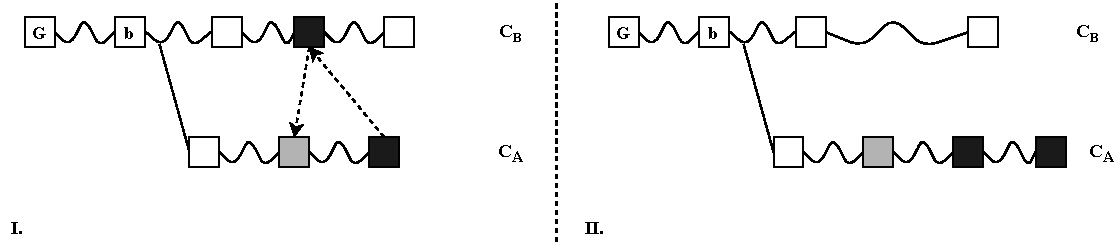
\includegraphics[scale=0.6]{figures/injection.png}
	\end{center}
	\caption{\textit{Adversarially generated blocks sewed from an honest player's chain into the adversary's suffix proof.v$C_A$ is the adversarial fork chain and $C_B$ is the chain of an honest player. Blocks generated by the adversary are colored black. Dashed arrows represent interlink pointers. Wavy lines imply one or more blocks. \textbf{I:} The real picture
	 of the chains. \textbf{II:} Equivalent picture considering the hashing power included in the corresponding suffix proof of each chain.}}
	\label{fig:injection}
\end{figure}


\section{Security Proof}
Our security proof is based on the security proof of NIPoPoWs Suffix Security Proof under a soft or hard fork. Consequently, most of the Definitions and Lemmas presented in Section \ref{proof_under_hard_fork} will be referenced and applied for the security proof under velvet fork conditions.
Our working hypothesis is that we operate under honest majority considering only the updated players. This is formally described in the following definition.\\
\textbf{Honest Majority Assumption under Velvet Fork Conditions.} A number of $t'$ out of $n'$ upgraded parties are corrupted such that $t' \leq (1 - \delta)(n' - t')$, where parameter $\delta$ is defined as in the Bitcoin Backbone paper \cite{Backbone}.\\
\textbf{Theorem 3. (Security under velvet fork)} \textit{Assuming honest majority under velvet fork conditions, the non-interactive proofs-of-proof-of-work construction for computable $\kappa$-stable monotonic suffix-sensitive predicates under velvet fork conditions is secure with overwhelming probability in $\kappa$.}\\
By contradiction. We follow the construction of Theorem 2 proof and extend it. Let $Q$ be a $\kappa-$stable monotonic suffix-sensitive chain predicate. Assume NIPoPoWs under velvet fork on $Q$ is insecure. Then, during an execution at some round  $r_3$, $Q(C)$ is defined and the verifier $V$ disagrees with some honest participant. Assume the execution is typical. $V$ communicates with adversary $A$ and honest prover $B$. The verifier receives proofs $\pi_A, \pi_B$. Because $B$ is honest, $\pi_B$ is a proof constructed based on underlying blockchain $C_B$ (with $\pi_B \subseteq C_B$), which $B$ has adopted during round $r_3$ at which $\pi_B$ was generated. Consider $C_A$ the chain containing at least some of the blocks in $\pi_A$, while the remaining blocks $\pi_A$ must belong in the $C_B$. 
The verifier outputs $\neg Q(C_B)$. Thus it is necessary that $\pi_A \geq \pi_B$. We show that $\pi_A \geq \pi_B$ is a negligible event. 
Let $b = LCA(\pi_A, \pi_B)$. Let the levels of comparison decided by the verifier be $\mu_A$ and $\mu_B$ respectively. Let $\mu'_B$ be the adequate level of proof $\pi_B$  with respect to block $b$. Call $\alpha_A = \pi_A \uparrow^{\mu_A}\{b:\}$, 
$\alpha'_B = \pi_B \uparrow^{\mu'_B}\{b:\}$.\\
The above are illustrated, among other, in Parts I, II of Figure \ref{fig:proof_velvet}.
\begin{figure}[h!]
	\begin{center}
		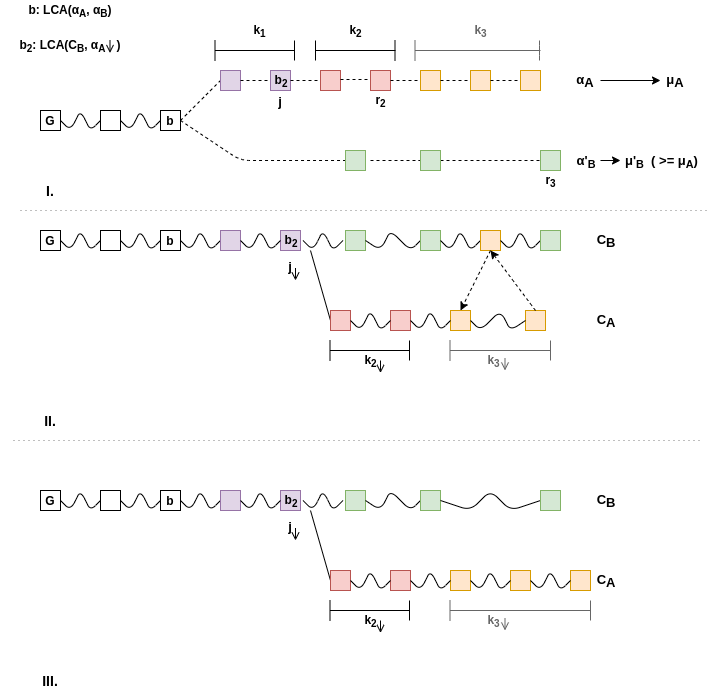
\includegraphics[scale=0.5]{figures/proof_velvet.png}
	\end{center}
	\caption{\textit{ Wavy lines imply one or more blocks. Dashed lines and arrows imply interlink pointers to superblocks. \textbf{I}: the three round sets in two competing proofs at different levels, \textbf{II}: the corresponding 0-level chains, \textbf{III}: the reformed chains $C_B$, $C_A$ so that adversarially generated blocks with false interlink participating in cyclic dependency with $C_A$ are removed from $C_B$ and added to $C_A$.}}
	\label{fig:proof_velvet}
\end{figure}
We will now show three successive claims under velvet fork conditions: First, $\alpha_A \downarrow \uparrow^{\mu_A}$ and $\alpha'_B \downarrow$ are mostly disjoint. Second, $a_A$ contains mostly adversarially generated blocks. And third, the adversary is able to produce this $a_A$ with negligible probability. Note that the notation $\alpha_A \downarrow \uparrow^{\mu_A}$ denotes the blocks of $\alpha_A$ which belong in the 0-level chain $C_A$, thus are not sewed in the adversary's proof by $C_B$.\\
Let $\alpha_A = k_1 + k_2 + k_3$ and let $k_1, k_2, k_3$ be as defined in the following Claims.\\
Let round $r_1$ be the round when block $b$ is generated and round $r_2$ when block $b_2 = LCA(\alpha_A \downarrow \uparrow^{\mu_A}, \alpha'_B\downarrow)$ is generated.\\
\textbf{Claim 1:} $\alpha_A \downarrow \uparrow^{\mu_A}, \alpha'_B\downarrow$ are mostly disjoint. Following the proof of Theorem 2 we conclude that $\vert \alpha_A\downarrow\uparrow^{\mu_A}[1:] \cap \alpha'_B\downarrow[1:] \vert \leq k_{1} = 2^{\mu'_B - \mu_A}$. In order to see this under the velvet fork conditions consider the following two claims. First let block $b_2 = LCA(\alpha_A \downarrow \uparrow^{\mu_A}, \alpha'_B\downarrow)$. This means that $b_2$ is the LCA block considering the adversary's proof and honest player's 0-level chain excluding any adversarially generated block included in $\alpha_A$ after the 0-level fork point.\\
\textit{\underline{Claim 1a}:} If no adversarially generated block of chain $C_B$ with incorrect interlink is included in $\alpha_A$ until block $b_2$ then the claim's proof is the same to that of Theorem 2, thus we have $k_1 \leq 2^{\mu'_B - \mu_A}$.\\
\textit{\underline{Claim 1b}:}  If a block $b' = \{b' \in C_B\{b:b_2\} \cap \textit{ } b' \textit{ contains incorrect interlink} \}$ is included in $\alpha_A$ then we have that $\vert \alpha_A\downarrow\uparrow^{\mu_A}[1:] \cap \alpha'_B\downarrow[1:] \vert \leq k_1 = k_{1a} + k_{1b}$, where $ k_{1a} = 2^{\mu'_B - \mu_A}$. 
	
Note that after block $b'$ no more honestly generated blocks of the common subchain $C_B\{b':b_2\}$ are included in $\alpha_A$ because of Remark 2. Blocks in $\alpha_A\{b':b_2\}$ are all adversarially generated of $C_B$. Thus from that point on it is equivalent considering two disjoint chains, one with honestly and another with adversarially generated blocks, competing each other. Let these adversarially generated blocks count to $k_{1b}$,  where $k_{1b} \leq C_B\{b':b_2\}\uparrow^{\mu_A}$.\\ \textit{(In the end, consider the rounds when these blocks were generated and apply Lemma 1 to get a desirable inequality)}\\
From all the above, we conclude that there are $\vert \alpha_A \vert - k_1$ blocks after block $b$ in $\alpha_A$ which are not honestly generated blocks existing in $\alpha_B\downarrow$. In other words, there are $\vert \alpha_A \vert - k_1$ blocks after block $b$ in $\alpha_A$, which are either adversarially generated existing in $\alpha_B\downarrow$ either don't belong in $\alpha_B\downarrow$. This makes $b_2$ the last block before the 0-level fork point included in the adversary's proof.\\
\textbf{Claim 2.} 
At least $k_3$ superblocks of $\alpha_A$ are adversarially generated. Just as the proof of Theorem 2 and using a similar notation, because of the Common Prefix property on parameter $k_{2a\downarrow}$, $\alpha_A \downarrow \uparrow [k_{1a}+k_{2a}:]$ could contain no honestly generated blocks. In case there are no sewed blocks, the above holds for $\alpha_A$ too. In order to generalize to velvet fork conditions, let the sewed blocks count to $k_{2b}$ and the sum $k_2 = k_{2a} + k_{2b}$. We conclude that $\alpha_A [k_{1}+k_{2}:]$ could contain no honestly generated blocks. \\ 
Note that for every sewed subchain the adversary includes in her proof, it may be that some other blocks generated in the adversary's chain are left out of the proof. This is due to the way blocks are generated in order to form a valid chain. So, in a case where a number of $C_B$ blocks are sewed in $C_A$ between blocks $b_{s_1}$ and $b_{s_2}$, say at rounds $s_1, s_2$ accordingly, any block generated in $C_A$ in the round set $s_1..s_2$ would be left out of the proof. This is illustrated in Figure \ref{fig:exclude}.\\
\begin{figure}[h!]
	\begin{center}
		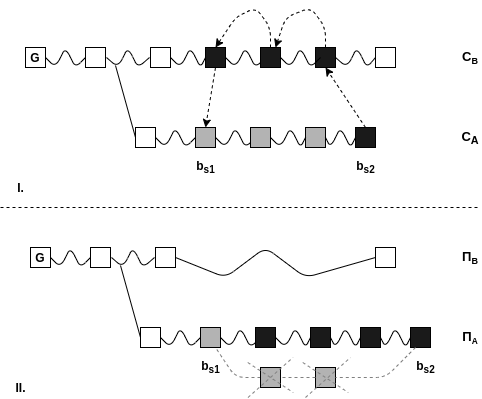
\includegraphics[scale=0.5]{figures/exclude.png}
	\end{center}
	\caption{\textit{ Wavy lines imply one or more blocks. Dashed arrows imply interlink pointers to superblocks. Adversarially generated blocks are colored black. Grey colored blocks may be honestly or adversarially generated. \textbf{I}: the 0-level chains, \textbf{II}: the corresponding proof chains; some blocks generated in $C_A$ are excluded from proof $\pi_A$ in favor of the sewed blocks from $C_B$.}}
	\label{fig:exclude}
\end{figure}
%
%Claim * calculates an upper bound of the adversarially generated blocks that $\alpha_A, \alpha'_B\downarrow$ may have in common.\\
%\textit{\underline{Claim *}:} Now consider the blocks containing incorrect interlink. By the time such a block is included in $\alpha_A$, then no other honestly generated block of chain $C_B$ will be included in $\alpha_A$ because of Remark 1 (no honestly generated block included in proof can point to a superblock containing false interlink). Thus, in that case it is equivalent to consider two different chains, the one of the adversary and the other of the honest players, that compete each other. This case may appear after $k_{1a}$ blocks in the $\alpha_A$ as described in the above Claims. Let $b_1 = \{GCA(C_B, \alpha_A) \cap b_1 \textit{ contains false interlink}\}$ and block $b_2 = LCA(C_B, \alpha_A)$. Thus we have 
%$\vert \alpha_A[1:] \cap \alpha'_B\downarrow[1:] \vert = k_{1a} + k_{1b}$, where $k_{1b} \leq C_B\{b_1:b_2\}\uparrow^{\mu_A}$.\\
In the following we consider the reformed chains $C_A, C_B$ for blocks in the $k_3$ region of the proofs. This reforming suggests the following: all adversarially generated blocks with false interlink in subchain $C_B\{b_2:\}$ which participate in cyclic dependency with fork chain $C_A$, are removed from $C_B$ and added in $C_A$ just as the interlink pointers forming the cyclic dependency point out. This reforming is helpful for the purposes of our proof construction and does not change the facts of the problem, or put it in another way, gives us an equivalent problem to solve. This is true, because of Remark 1, that such blocks cannot be included in an honest NIPoPoW proof while can be included in the proof constructed by the adversary, thus from the NIPoPoW suffix proofs perspective these block can be perceived as belonging in the adversary's fork chain. This remark is considered in the following Claim.\\
\textbf{Claim 3.} We reform the chains $C_A, C_B$ as illustrated in Figure 5 (I, II) and Figure \ref{fig:claim3} (II, III). After this reforming we conclude to an equivalent set of compared subchains. Note that the problems before and after the reforming are equivalent because of Remarks 1 and 2. Then this Claim is exactly the same as that of Theorem 2.
In order to complete the proof we work in the same way as in Theorem 2, by considering the three parts of $\alpha_A$ proof ....
From all the above Claims we have that:\\
In the first round set, because of the common underlying chain:
\begin{equation*}
2^{\mu_A} \vert \alpha_A^{k_{1a}} \vert \leq 2^{\mu'_B} \vert \alpha'{_B^{k_{1a}}} \vert
\end{equation*}
and because of Lemma 1 we obtain with high probability:
\begin{equation*} 
2^{\mu_A} \vert \alpha_A^{k_{1b}} \vert \leq 2^{\mu'_B} \vert \alpha'{_B^{k_{1b}}} \vert
\end{equation*}
So finally:
\begin{equation} \label{eq_v_round_set_1}
2^{\mu_A} \vert \alpha_A^{k_1} \vert \leq 2^{\mu'_B} \vert \alpha'{_B^{k_1}} \vert
\end{equation}
In the second round set:\\
(To be completed.)\\
In the third round set, considering the equivalent problem after reforming the chains because of Honest Majority Assumption under Velvet Fork and Lemma 1 we have:
\begin{equation} \label{eq_v_round_set_3}
2^{\mu_A} \vert \alpha_A^{k_3} \vert < 2^{\mu'_B} \vert \alpha'{_B^{k_3}} \vert
\end{equation}

\subsection{Infix Proofs}

\bibliographystyle{plain} % We choose the "plain" reference style
\bibliography{refs} % Entries are in the "refs.bib" file

\end{document}